\documentclass[aspectratio=169, 10pt]{beamer}

\usepackage{bm} % bold math
\usepackage{fontspec}
\usepackage{minted}
\usepackage{pgf-pie}
\usepackage{tikz}

% Custom commands and environments
\makeatletter
\newcommand\version[1]{\renewcommand\@version{#1}}
\newcommand\@version{}
\def\insertversion{\@version}

\newcommand\course[1]{\renewcommand\@course{#1}}
\newcommand\@course{}
\def\insertcourse{\@course}

\newcommand\coursetitle[1]{\renewcommand\@coursetitle{#1}}
\newcommand\@coursetitle{}
\def\insertcoursetitle{\@coursetitle}

\newcommand\lecturenumber[1]{\renewcommand\@lecturenumber{#1}}
\newcommand\@lecturenumber{}
\def\insertlecturenumber{\@lecturenumber}
\makeatother

\newcommand{\slidetitle}[1]{{\xbseries \large \structure{#1}} \bigskip}
\newcommand{\term}[1]{{\color{blue} #1}}
\newcommand{\leftspace}{\hspace{1em}}
\newcommand{\inlinearrow}{
  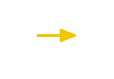
\begin{tikzpicture}[baseline]
    \node [anchor=base] (x) {};
    \draw [rawarrow] (x.mid west) -- ($(x.mid west) + (2em,0)$);
  \end{tikzpicture}
}

\newenvironment{slide}
{\begin{frame}[fragile,environment=slide]\vskip0pt plus 1filll}
{\vskip0pt plus 1filll\end{frame}}

% LaTeX

\setlength{\leftmargini}{1em}

% Common Information

\author{Jon Eyolfson}
\course{ECE 353}
\coursetitle{Systems Software}
\date{2024 Winter}

% fontspec

\defaultfontfeatures{Ligatures=TeX}
% \setmainfont{Domine}
\setsansfont{Inter}[
  FontFace={ul}{n}{Font=*-Thin},
  FontFace={el}{n}{Font=*-ExtraLight},
  FontFace={l}{n}{Font=*-Light},
  FontFace={sb}{n}{Font=*-SemiBold},
  FontFace={eb}{n}{Font=*-ExtraBold},
  FontFace={xb}{n}{Font=*-Black},
]
\setmonofont[Contextuals=AlternateOff, Ligatures=TeXOff]{Iosevka}[
  FontFace={xb}{n}{Font=*-Heavy},
]

%% Font Weights

\DeclareRobustCommand{\ulseries}{\fontseries{ul}\selectfont}
\DeclareTextFontCommand{\textul}{\ulseries}
\DeclareRobustCommand{\elseries}{\fontseries{el}\selectfont}
\DeclareTextFontCommand{\textel}{\elseries}
\DeclareRobustCommand{\lseries}{\fontseries{l}\selectfont}
\DeclareTextFontCommand{\textl}{\lseries}
\DeclareRobustCommand{\sbseries}{\fontseries{sb}\selectfont}
\DeclareTextFontCommand{\textsb}{\sbseries}
\DeclareRobustCommand{\ebseries}{\fontseries{eb}\selectfont}
\DeclareTextFontCommand{\texteb}{\ebseries}
\DeclareRobustCommand{\xbseries}{\fontseries{xb}\selectfont}
\DeclareTextFontCommand{\textxb}{\xbseries}

% tikz

\usetikzlibrary{
  arrows,
  arrows.meta,
  automata,
  backgrounds,
  calc,
  decorations.pathreplacing,
  matrix,
  positioning,
  overlay-beamer-styles,
  shapes,
  shapes.multipart,
  tikzmark,
}

\tikzstyle{rawarrow} = [
  -{Latex[round]},
  line width=1pt,
  yellow,
  shorten >=3pt,
  shorten <=3pt,
  font=\small,
  text=black,
]

\tikzstyle{arrow} = [
  -{Latex[round]},
  line width=1pt,
  yellow,
  shorten >=3pt,
  shorten <=3pt,
  transform canvas={yshift=3pt},
  font=\small,
  text=black,
]

\newcommand{\tikzmarkcoord}[1]{([yshift=3pt]pic cs:#1)}

% minted

\setminted{style=eyolfson, fontsize=\small, escapeinside=||}
\setmintedinline{fontsize=\normalsize}

% hyperref

\hypersetup{colorlinks, urlcolor=blue}

% beamer
\setbeamersize{text margin left=16mm, text margin right=16mm}
\setbeamertemplate{itemize items}[circle]
\setbeamercolor{item}{fg=black}
\setbeamercolor{structure}{fg=darkblue}
\setbeamerfont{frametitle}{series=\bfseries, parent=structure}
\setbeamertemplate{navigation symbols}{}
\setbeamertemplate{headline}{}
\setbeamertemplate{footline}{
  \begin{tikzpicture}[
    remember picture,
    overlay,
    shift={(current page.south west)},
  ]
    \path [fill=gray] (144mm, 0) -- (160mm, 16mm) -- (160mm, 0);
    \node [inner sep=3.5mm, outer sep=0, text=black, anchor=base east,
           align=right, yshift=3.5mm]
          at (current page.south east) {\ttfamily \small \insertframenumber{}};
  \end{tikzpicture}
}
\setbeamertemplate{title page}{
  \begin{tikzpicture}[
    remember picture,
    overlay,
    shift={(current page.south west)},
    background rectangle/.style={fill=darkblue},
    show background rectangle,
  ]
    \node [anchor=center, align=center, text=white, text width=40mm, scale=3.2]
          at (\paperwidth / 2, \paperheight * 2 / 3)
          {\xbseries \inserttitle{}};
    \node [anchor=base west, align=left, inner sep=0, text=white, yshift=2.5mm]
          at (16mm, \paperheight / 3)
          {\insertdate{} \insertcourse{}: \insertcoursetitle{}};
    \node [anchor=base west, align=left, inner sep=0, text=white, yshift=-2.5mm]
          at (16mm, \paperheight / 3)
          {\insertauthor};
    \node [anchor=base east, align=right, inner sep=0, text=white, yshift=2.5mm]
          at (144mm, \paperheight / 3)
          {Lecture \insertlecturenumber{}};
    \node [anchor=base east, align=right, inner sep=0, text=white,
           yshift=-2.5mm]
          at (144mm, \paperheight / 3)
          {\ttfamily \insertversion{}};
    \node [align=center, anchor=south, inner sep=0, text=white, yshift=3.5mm]
          (license) at (\paperwidth / 2, 0)
          {\fontsize{7pt}{7pt}\selectfont This  work is licensed under a
           \href{http://creativecommons.org/licenses/by-sa/4.0/}
                {\color{lightblue} Creative Commons Attribution-ShareAlike 4.0
                 International License}};
  \end{tikzpicture}
}

% xcolor

%% Primary Colour

\definecolor{pantone655}{RGB}{0, 42, 92} % #002a5c
\colorlet{darkblue}{pantone655}

%% Secondary Colours

\definecolor{pantone633}{RGB}{0, 139, 176} % #008bb0
\colorlet{blue}{pantone633}

\definecolor{pantonewarmred}{RGB}{220, 70, 51} % #dc4633
\colorlet{red}{pantonewarmred}

\definecolor{pantone3285}{RGB}{0, 161, 137} % #00a189
\colorlet{cyan}{pantone3285}

\definecolor{pantone7722}{RGB}{13, 83, 77} % #0d534d
\colorlet{darkcyan}{pantone7722}

\definecolor{pantone376}{RGB}{141, 191, 46} % #8dbf2e
\colorlet{green}{pantone376}

\definecolor{pantone2613}{RGB}{109, 36, 122} % #6d247a
\colorlet{violet}{pantone2613}

\definecolor{pantone2985}{RGB}{111, 199, 234} % #6fc7ea
\colorlet{lightblue}{pantone2985}

\definecolor{pantone227}{RGB}{171, 19, 104} % #ab1368
\colorlet{magenta}{pantone227}

\definecolor{pantone7406}{RGB}{241, 197, 0} % #f1c500
\colorlet{yellow}{pantone7406}

%% Neutrals

\definecolor{pantonecoolgray2}{RGB}{208, 209, 201} % #d0d1c9
\colorlet{gray}{pantonecoolgray2}


\lecturenumber{29}
\title{Page Replacement}
\version{2.0.1}

\usetikzlibrary{intersections} % /tikz/name path

\tikzset{swapin/.style args = {(#1,#2)}{%
    row #1 column #2/.style={nodes={text=red}}}}

\begin{document}

  \begin{frame}[plain, noframenumbering]
    \titlepage
  \end{frame}

  \begin{slide}
    
    \slidetitle{
      Computer Memory Hierarchy is a
    
      Trade-off of Capacity and Speed
    }

    \centering
    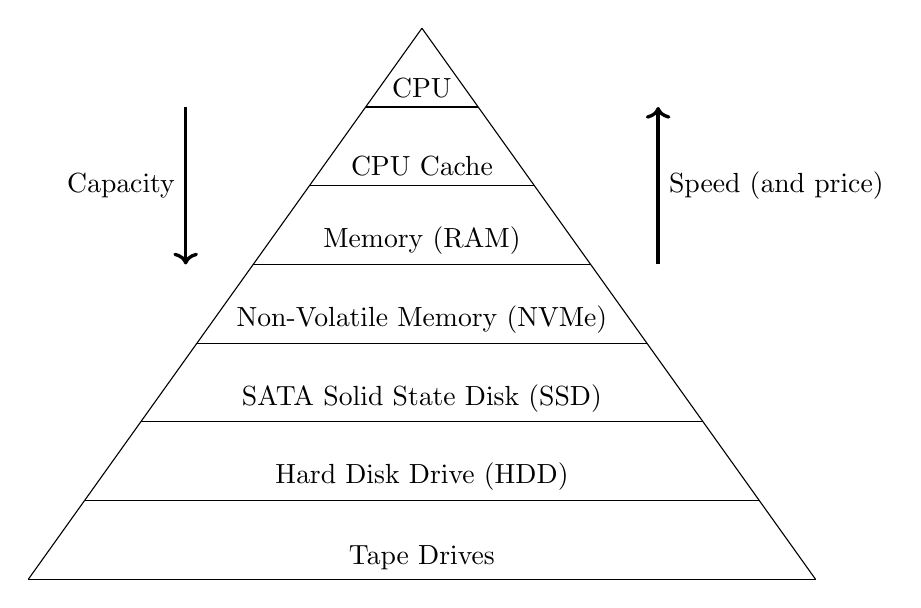
\begin{tikzpicture}[shorten >=0pt]
      \coordinate (A) at (-5,0) {};
      \coordinate (B) at ( 5,0) {};
      \coordinate (C) at (0,7) {};
      \draw[name path=AC] (A) -- (C);
      \draw[name path=BC] (B) -- (C);
      \foreach \y/\A in {
        0/Tape Drives,
        1/Hard Disk Drive (HDD),
        2/SATA Solid State Disk (SSD),
        3/Non-Volatile Memory (NVMe),
        4/Memory (RAM),
        5/CPU Cache,
        6/CPU
      } {
        \draw ($(A)!\y/7!(C)$) -- ($(B)!\y/7!(C)$)
          node[midway,above] {\A};
      }

      \draw [->, very thick] (-3,6) -- (-3,4) node[midway, left] {Capacity};
      \draw [->, very thick] (3,4) -- (3,6) node[midway, right] {Speed (and price)};
    \end{tikzpicture}

  \end{slide}

  \begin{slide}

    \slidetitle{We Want to Hide the Hierarchy from the User}

    Each level wants to pretend it has the speed of the layer above it

    \leftspace{}and the capacity of the layer below it
    \medskip

    The memory used by all the processes my exceed the amount of physical memory

    \leftspace{}Not all of them may be in use at the same time
    \medskip

    Only keep referenced pages in memory, put others on disk

    \leftspace{}Swap pages back to memory when they're needed

  \end{slide}

  \begin{slide}

    \slidetitle{Demand Paging}

    We use memory as a cache for the file system
    \medskip

    Map memory pages to file system blocks

    \leftspace{}Only load them into memory when they're used through
    the page fault handler
    \medskip

    If the page doesn't represent a file, we can map it to swap space

    \leftspace{}Move it to disk if we need to use more physical memory

  \end{slide}

  \begin{slide}

    \slidetitle{A Processes' Working Set Should Fit in Physical Memory}

    Given an amount of time, the number of pages your process uses
    is called
    its \textit{working set}
    \medskip

    If you cannot fit your working set into physical memory your process
    will \textit{thrash}

    \leftspace{}It's constantly moving entries in and out of cache

  \end{slide}

  \begin{slide}

    \slidetitle{Page Replacement Algorithms}

    Optimal

    \leftspace{}Replace the page that won't be used for the longest
    \medskip

    Random

    \leftspace{}Replace a random page
    \medskip

    First-in First-out (FIFO)

    \leftspace{}Replace the oldest page first
    \medskip

    Least Recently Used (LRU)

    \leftspace{}Replace the page that hasn't been used in the longest time

  \end{slide}

  \begin{slide}

    \slidetitle{Page Replacement Evaluation}

    Assume our physical memory can only hold 4 pages, and we access the following:

    \leftspace{}1 2 3 4 1 2 5 1 2 3 4 5 (all of the pages are initially on disk)
    \medskip

    We'll use this for a bunch of examples during this lecture

    \leftspace{}We want the fewest number of page faults
    \medskip

    For every example we'll find the number of page faults

  \end{slide}

  \begin{slide}

    \slidetitle{Optimal Example}

    Assume our physical memory can only hold 4 pages, and we access the following:

    \leftspace{}1 2 3 4 1 2 5 1 2 3 4 5 (all of the pages are initially on disk)

    \begin{center}
      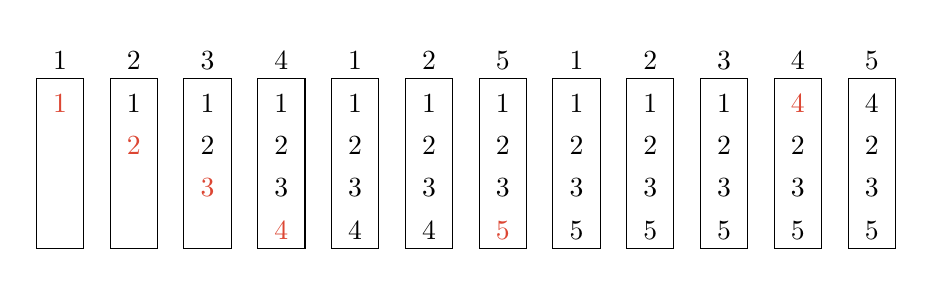
\begin{tikzpicture}[
        every node/.style={
          align=center,
          text height=2ex,
          text width=1em
        },
        swapin/.list={
          (2,1),
          (3,2),
          (4,3),
          (5,4),
          (5,7),
          (2,11)
        },
      ]
        \matrix (m) [
          matrix of nodes,
          nodes in empty cells,
          column sep=1em,
          column 2/.style={visible on=<2->},
          column 3/.style={visible on=<3->},
          column 4/.style={visible on=<4->},
          column 5/.style={visible on=<5->},
          column 6/.style={visible on=<6->},
          column 7/.style={visible on=<7->},
          column 8/.style={visible on=<8->},
          column 9/.style={visible on=<9->},
          column 10/.style={visible on=<10->},
          column 11/.style={visible on=<11->},
          column 12/.style={visible on=<12->},
        ] {
          1 & 2 & 3 & 4 & 1 & 2 & 5 & 1 & 2 & 3 & 4 & 5 \\
          1 & 1 & 1 & 1 & 1 & 1 & 1 & 1 & 1 & 1 & 4 & 4 \\
            & 2 & 2 & 2 & 2 & 2 & 2 & 2 & 2 & 2 & 2 & 2 \\
            &   & 3 & 3 & 3 & 3 & 3 & 3 & 3 & 3 & 3 & 3 \\
            &   &   & 4 & 4 & 4 & 5 & 5 & 5 & 5 & 5 & 5 \\
        };
        \draw (m-2-1.north west) rectangle (m-5-1.south east);
        \draw (m-2-2.north west) rectangle (m-5-2.south east);
        \draw (m-2-3.north west) rectangle (m-5-3.south east);
        \draw (m-2-4.north west) rectangle (m-5-4.south east);
        \draw (m-2-5.north west) rectangle (m-5-5.south east);
        \draw (m-2-6.north west) rectangle (m-5-6.south east);
        \draw (m-2-7.north west) rectangle (m-5-7.south east);
        \draw (m-2-8.north west) rectangle (m-5-8.south east);
        \draw (m-2-9.north west) rectangle (m-5-9.south east);
        \draw (m-2-10.north west) rectangle (m-5-10.south east);
        \draw (m-2-11.north west) rectangle (m-5-11.south east);
        \draw (m-2-12.north west) rectangle (m-5-12.south east);
      \end{tikzpicture}
    \end{center}

    \begin{flushright}
      \onslide<13->{6 page faults}
    \end{flushright}

  \end{slide}

  \begin{slide}

    \slidetitle{FIFO Example}

    Assume our physical memory can only hold 4 pages, and we access the following:

    \leftspace{}1 2 3 4 1 2 5 1 2 3 4 5 (all of the pages are initially on disk)

    \begin{center}
      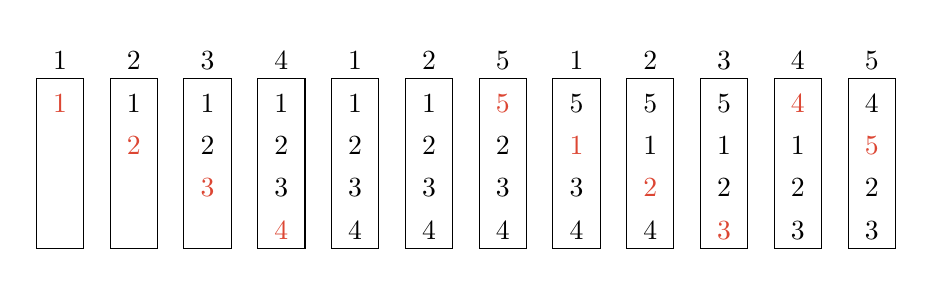
\begin{tikzpicture}[
        every node/.style={
          align=center,
          text height=2ex,
          text width=1em
        },
        swapin/.list={
          (2,1),
          (3,2),
          (4,3),
          (5,4),
          (2,7),
          (3,8),
          (4,9),
          (5,10),
          (2,11),
          (3,12)
        },
      ]
        \matrix (m) [
          matrix of nodes,
          nodes in empty cells,
          column sep=1em,
          column 2/.style={visible on=<2->},
          column 3/.style={visible on=<3->},
          column 4/.style={visible on=<4->},
          column 5/.style={visible on=<5->},
          column 6/.style={visible on=<6->},
          column 7/.style={visible on=<7->},
          column 8/.style={visible on=<8->},
          column 9/.style={visible on=<9->},
          column 10/.style={visible on=<10->},
          column 11/.style={visible on=<11->},
          column 12/.style={visible on=<12->},
        ] {
          1 & 2 & 3 & 4 & 1 & 2 & 5 & 1 & 2 & 3 & 4 & 5 \\
          1 & 1 & 1 & 1 & 1 & 1 & 5 & 5 & 5 & 5 & 4 & 4 \\
            & 2 & 2 & 2 & 2 & 2 & 2 & 1 & 1 & 1 & 1 & 5 \\
            &   & 3 & 3 & 3 & 3 & 3 & 3 & 2 & 2 & 2 & 2 \\
            &   &   & 4 & 4 & 4 & 4 & 4 & 4 & 3 & 3 & 3 \\
        };
        \draw (m-2-1.north west) rectangle (m-5-1.south east);
        \draw (m-2-2.north west) rectangle (m-5-2.south east);
        \draw (m-2-3.north west) rectangle (m-5-3.south east);
        \draw (m-2-4.north west) rectangle (m-5-4.south east);
        \draw (m-2-5.north west) rectangle (m-5-5.south east);
        \draw (m-2-6.north west) rectangle (m-5-6.south east);
        \draw (m-2-7.north west) rectangle (m-5-7.south east);
        \draw (m-2-8.north west) rectangle (m-5-8.south east);
        \draw (m-2-9.north west) rectangle (m-5-9.south east);
        \draw (m-2-10.north west) rectangle (m-5-10.south east);
        \draw (m-2-11.north west) rectangle (m-5-11.south east);
        \draw (m-2-12.north west) rectangle (m-5-12.south east);
      \end{tikzpicture}
    \end{center}

    \begin{flushright}
      \onslide<13->{10 page faults}
    \end{flushright}

  \end{slide}

  \begin{slide}

    \slidetitle{FIFO Example (3 Page Frames)}

    Assume our physical memory can only hold \textbf{3} pages, and we access the following:

    \leftspace{}1 2 3 4 1 2 5 1 2 3 4 5 (all of the pages are initially on disk)

    \begin{center}
      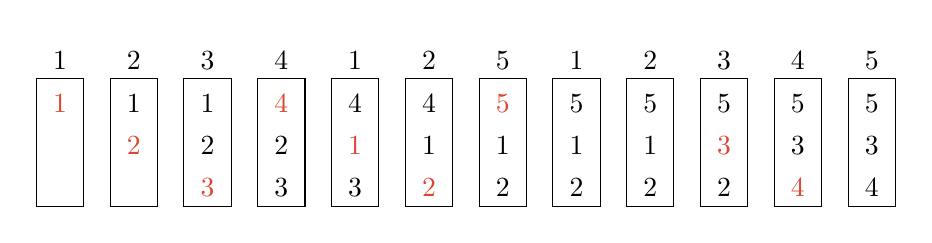
\begin{tikzpicture}[
        every node/.style={
          align=center,
          text height=2ex,
          text width=1em
        },
        swapin/.list={
          (2,1),
          (3,2),
          (4,3),
          (2,4),
          (3,5),
          (4,6),
          (2,7),
          (3,10),
          (4,11)
        },
      ]
        \matrix (m) [
          matrix of nodes,
          nodes in empty cells,
          column sep=1em,
          column 2/.style={visible on=<2->},
          column 3/.style={visible on=<3->},
          column 4/.style={visible on=<4->},
          column 5/.style={visible on=<5->},
          column 6/.style={visible on=<6->},
          column 7/.style={visible on=<7->},
          column 8/.style={visible on=<8->},
          column 9/.style={visible on=<9->},
          column 10/.style={visible on=<10->},
          column 11/.style={visible on=<11->},
          column 12/.style={visible on=<12->},
        ] {
          1 & 2 & 3 & 4 & 1 & 2 & 5 & 1 & 2 & 3 & 4 & 5 \\
          1 & 1 & 1 & 4 & 4 & 4 & 5 & 5 & 5 & 5 & 5 & 5 \\
            & 2 & 2 & 2 & 1 & 1 & 1 & 1 & 1 & 3 & 3 & 3 \\
            &   & 3 & 3 & 3 & 2 & 2 & 2 & 2 & 2 & 4 & 4 \\
        };
        \draw (m-2-1.north west) rectangle (m-4-1.south east);
        \draw (m-2-2.north west) rectangle (m-4-2.south east);
        \draw (m-2-3.north west) rectangle (m-4-3.south east);
        \draw (m-2-4.north west) rectangle (m-4-4.south east);
        \draw (m-2-5.north west) rectangle (m-4-5.south east);
        \draw (m-2-6.north west) rectangle (m-4-6.south east);
        \draw (m-2-7.north west) rectangle (m-4-7.south east);
        \draw (m-2-8.north west) rectangle (m-4-8.south east);
        \draw (m-2-9.north west) rectangle (m-4-9.south east);
        \draw (m-2-10.north west) rectangle (m-4-10.south east);
        \draw (m-2-11.north west) rectangle (m-4-11.south east);
        \draw (m-2-12.north west) rectangle (m-4-12.south east);
      \end{tikzpicture}
    \end{center}

    \begin{flushright}
      \onslide<13->{9 page faults}
    \end{flushright}

  \end{slide}

  \begin{slide}

    \slidetitle{Bélády's Anomaly Says More Page Frames Causes More Faults}

    This is a problem with FIFO algorithms

    \leftspace{}Does not exist with LRU or ``stack-based algorithms''
    \medskip

    Paper in 2010 found that this FIFO anomaly is unbounded (\url{https://arxiv.org/abs/1003.1336})

    \leftspace{}You could construct a sequence to get any arbitrary page fault ratio
    \medskip

    For other algorithms:

    \leftspace{}increasing the number of page frames decreases the number of
    page faults

  \end{slide}

  \begin{slide}

    \slidetitle{LRU Example (Use FIFO to Break Ties)}

    Assume our physical memory can only hold 4 pages, and we access the following:

    \leftspace{}1 2 3 4 1 2 5 1 2 3 4 5 (all of the pages are initially on disk)

    \begin{center}
      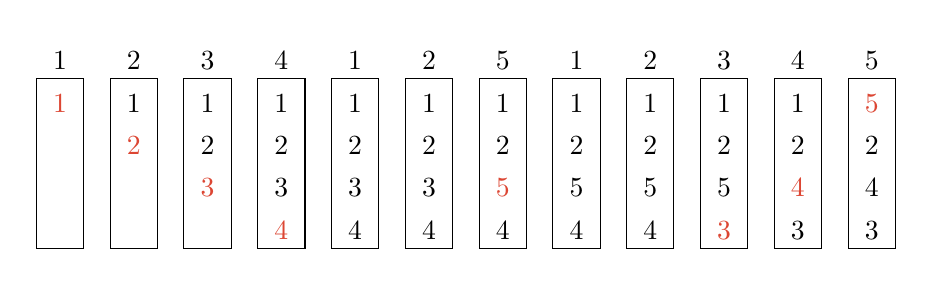
\begin{tikzpicture}[
        every node/.style={
          align=center,
          text height=2ex,
          text width=1em
        },
        swapin/.list={
          (2,1),
          (3,2),
          (4,3),
          (5,4),
          (4,7),
          (5,10),
          (4,11),
          (2,12)
        },
      ]
        \matrix (m) [
          matrix of nodes,
          nodes in empty cells,
          column sep=1em,
          column 2/.style={visible on=<2->},
          column 3/.style={visible on=<3->},
          column 4/.style={visible on=<4->},
          column 5/.style={visible on=<5->},
          column 6/.style={visible on=<6->},
          column 7/.style={visible on=<7->},
          column 8/.style={visible on=<8->},
          column 9/.style={visible on=<9->},
          column 10/.style={visible on=<10->},
          column 11/.style={visible on=<11->},
          column 12/.style={visible on=<12->},
        ] {
          1 & 2 & 3 & 4 & 1 & 2 & 5 & 1 & 2 & 3 & 4 & 5 \\
          1 & 1 & 1 & 1 & 1 & 1 & 1 & 1 & 1 & 1 & 1 & 5 \\
            & 2 & 2 & 2 & 2 & 2 & 2 & 2 & 2 & 2 & 2 & 2 \\
            &   & 3 & 3 & 3 & 3 & 5 & 5 & 5 & 5 & 4 & 4 \\
            &   &   & 4 & 4 & 4 & 4 & 4 & 4 & 3 & 3 & 3 \\
        };
        \draw (m-2-1.north west) rectangle (m-5-1.south east);
        \draw (m-2-2.north west) rectangle (m-5-2.south east);
        \draw (m-2-3.north west) rectangle (m-5-3.south east);
        \draw (m-2-4.north west) rectangle (m-5-4.south east);
        \draw (m-2-5.north west) rectangle (m-5-5.south east);
        \draw (m-2-6.north west) rectangle (m-5-6.south east);
        \draw (m-2-7.north west) rectangle (m-5-7.south east);
        \draw (m-2-8.north west) rectangle (m-5-8.south east);
        \draw (m-2-9.north west) rectangle (m-5-9.south east);
        \draw (m-2-10.north west) rectangle (m-5-10.south east);
        \draw (m-2-11.north west) rectangle (m-5-11.south east);
        \draw (m-2-12.north west) rectangle (m-5-12.south east);
      \end{tikzpicture}
    \end{center}

    \begin{flushright}
      \onslide<13->{8 page faults}
    \end{flushright}

  \end{slide}

  \begin{slide}

    \slidetitle{Implementing LRU in Hardware Has to Search All Pages}

    You could implement it by keeping a counter for each page
    \medskip

    For each page reference, save the system clock into the counter
    \medskip


    For replacement, scan through the pages and find the one with the oldest clock

  \end{slide}

  \begin{slide}

    \slidetitle{Implementing LRU in Software is Too Expensive}

    Create a doubly linked list of pages
    \medskip

    For each page reference, move it to the front of the list
    \medskip

    For replacement, remove from the back of the list
    \medskip

    It requires 6 pointer updates for each page reference, and

    \leftspace{}also creates a high contention bottleneck for multiple processors

  \end{slide}

  \begin{slide}

    \slidetitle{Implementing LRU in Practice Isn't Going to Work}

    We settle for approximate LRU

    \leftspace{}LRU is an approximation of the optimal case anyways
    \medskip

    There's lots of different tweaks you can do to implement it more efficiently
    \medskip

    We'll be looking at the clock algorithm, but there's also:

    \leftspace{}Least Frequently Used (LFU), 2Q, Adaptive Replacement Cache (ARC)

  \end{slide}

  \begin{slide}

    \slidetitle{Page Replacement Algorithms Aim to Reduce Page Faults}

    We saw the following:
    \begin{itemize}
      \item Optimal (good for comparison but not realistic)
      \item Random (actually works surprisingly well, avoids the worst case)
      \item FIFO (easy to implement but Bélády's anomaly)
      \item LRU (gets close to optimal but expensive to implement)
    \end{itemize}

  \end{slide}

\end{document}
